Para exemplificar estados e ações legais, vamos examinar uma fase principal em que o agente é o jogador ativo a partir do começo do turno. O estado $s_1$ é, no caso, o estado inicial. Os atributos $d_1, d_2$ dos estados estão suprimidos, pois são irrelevantes para o exemplo. Para este exemplo iremos supor que o oponente do agente não tem nenhuma carta em sua mão, campo de batalha ou cemitério, e ambos os jogadores têm 10 pontos de vida.

\vskip1ex

\textbf{Figura E.1.1:} estado $s_1$

\begin{mdframed}
    \begin{center}
    $s_1 = \left\{ v_1 = v_2 = 10, h_1 = 4, h_2 = 0, B_2 = G_1 = G_2 = \emptyset, B_1, H \right\}$\\
    $R(s_1) = 3,3 + 4 = 7,3$
    \vskip1ex
    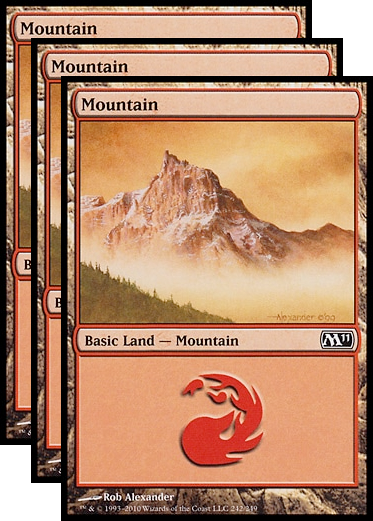
\includegraphics[width=0.2\textwidth]{picstcc/bf1.png}
    \vskip1ex
    $B_1$: O campo de batalha consiste apenas em 3 terrenos (Montanhas).

    \vspace{.1cm}

    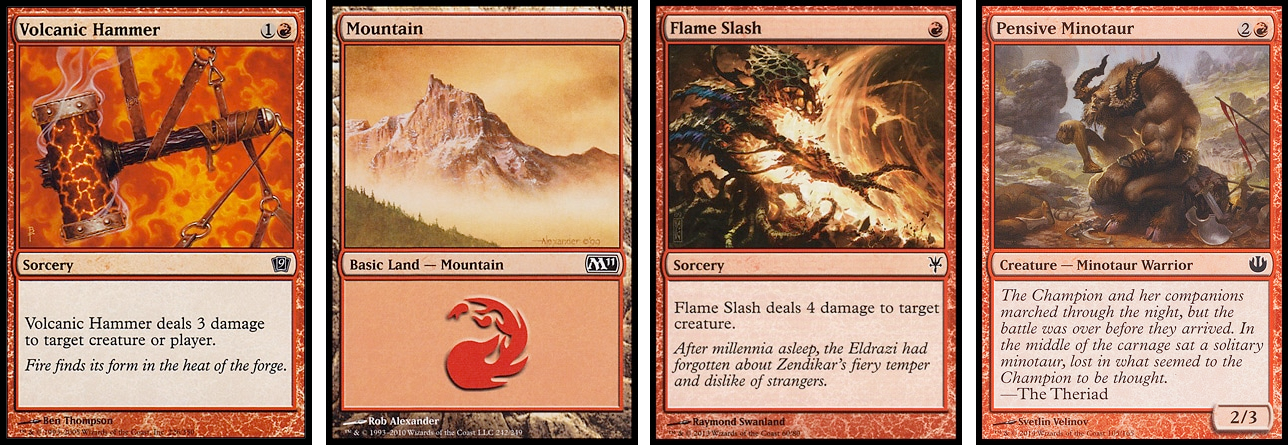
\includegraphics[width=0.9\textwidth]{picstcc/hand1.png}
    \vskip1ex
    $H$: A mão do agente consiste em um terreno (Montanha), um feitiço ``Volcanic Hammer'', um feitiço ``Flame Slash'' e uma criatura ``Pensive Minotaur''.

    \vskip1ex
    Dessa maneira, o conjunto de ações em $s_1$ pode ser definido a partir de $H$ e $B_1,B_2$:
    \begin{equation}
      A^P(s_1) := \begin{lrdcases}
                  Mountain \in Land, \\
                  PensiveMinotaur \in Creature(3), \\
                  VolcanicHammer(self) \in Sorcery(2, self), \\
                  VolcanicHammer(opponent) \in Sorcery(2, opponent), \\
                  Pass.
                  \end{lrdcases}
    \end{equation}
    Como não há criaturas em jogo, ``Flame Slash'' não tem alvos legais e não pode ser jogada. ``Volcanic Hammer'', por outro lado, admite ambos os jogadores como alvo válido, portanto pode ser jogada através de duas ações diferentes.
  \end{center}
\end{mdframed}

Suponhamos que o agente jogue a Montanha que tem na mão. Sendo assim, o estado $s_2$ é parecido com $s_1$.

\textbf{Figura E.1.2:} estado $s_2$

\begin{mdframed}
    \begin{center}
    $s_2 = \left\{ v_1 = v_2 = 10, h_1 = 3, h_2 = 0, B_2 = G_1 = G_2 = \emptyset, B_1, H \right\}$\\
    $R(s_2) = 4,4+3 = 7,4$
    \vskip1ex
    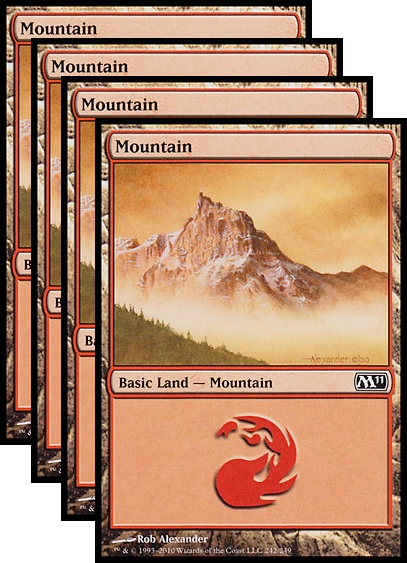
\includegraphics[width=0.2\textwidth]{picstcc/bf2.png}
    \vskip1ex
    $B_1$: O campo de batalha consiste apenas em 4 terrenos (Montanhas).

    \vspace{.1cm}

    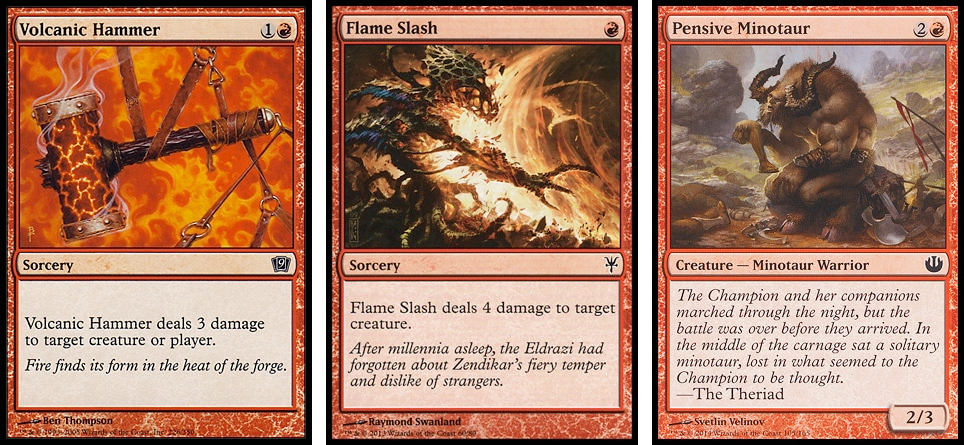
\includegraphics[width=0.9\textwidth]{picstcc/hand2.png}
    \vskip1ex
    $H$: A mão do agente consiste em um feitiço ``Volcanic Hammer'', um feitiço ``Flame Slash'' e uma criatura ``Pensive Minotaur''.

    \vskip1ex
    O conjunto de ações em $s_2$ é quase igual ao conjunto de ações em $s_1:$
    \begin{equation}
      A^P(s_2) := \begin{lrdcases}
                  PensiveMinotaur \in Creature(3), \\
                  VolcanicHammer(self) \in Sorcery(2, self), \\
                  VolcanicHammer(opponent) \in Sorcery(2, opponent), \\
                  Pass.
                  \end{lrdcases}
    \end{equation}
    ``Flame Slash'' ainda não pode ser jogada.
  \end{center}
\end{mdframed}

Agora, a ação escolhida em $s_2$ é jogar a carta ``Pensive Minotaur'', uma criatura sem efeitos. Para isso, é necessário virar 3 terrenos, alterando duplamente $B_1$.

\newpage
\textbf{Figura E.1.3:} estado $s_3$

\begin{mdframed}
    \begin{center}
    $s_3 = \left\{ v_1 = v_2 = 10, h_1 = 2, h_2 = 0, B_2 = G_1 = G_2 = \emptyset, B_1, H \right\}$\\
    $R(s_3) = 2 + 1,5 + 4,4 + 2 = 9,9$
    \vskip1ex
    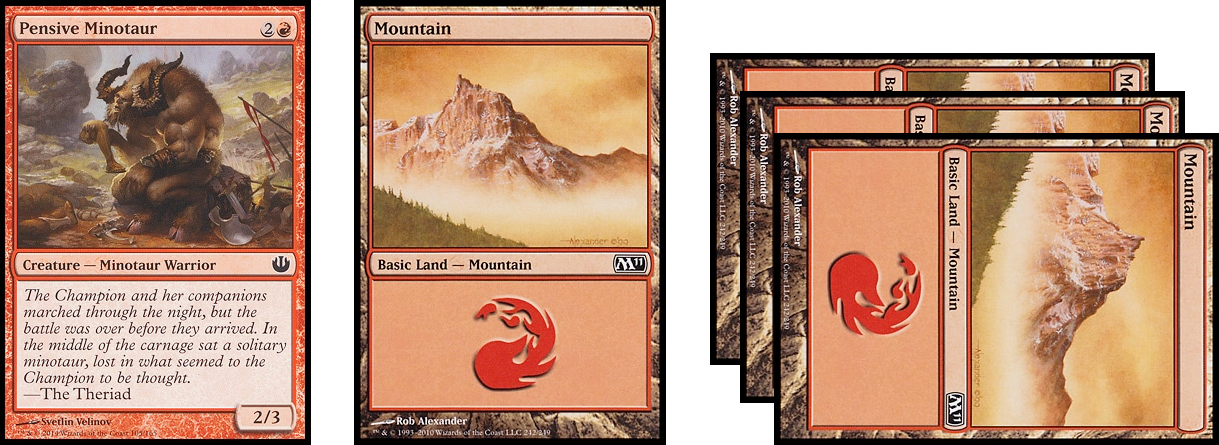
\includegraphics[width=0.6\textwidth]{picstcc/bf3.png}
    \vskip1ex
    $B_1$: Com ``Pensive Minotaur'' jogada, o campo de batalha agora contém ela, três montanhas viradas e uma montanha desvirada.

    \vspace{.1cm}

    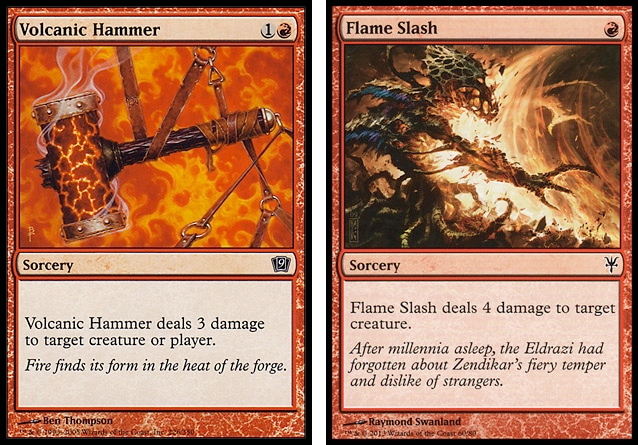
\includegraphics[width=0.7\textwidth]{picstcc/hand3.png}
    \vskip1ex
    $H$: A mão do agente consiste em um feitiço ``Volcanic Hammer'' e um feitiço ``Flame Slash''.

    \vskip1ex
    O conjunto de ações legais em $s_3$ muda radicalmente:
    \begin{equation}
      A^P(s_3) := \begin{lrdcases}
                  FlameSlash(Pensive Minotaur \in B_1) \in Sorcery(1, e \in B_1), \\
                  Pass.
                  \end{lrdcases}
    \end{equation}
    ``Flame Slash'' agora pode ser jogada.
  \end{center}
\end{mdframed}

Em $s_3$, como o agente tem apenas um terreno desvirado em jogo, jogar ``Volcanic Hammer'' em qualquer alvo passam a ser ações ilegais (pois são necessários dois terrenos para isso). Por outro lado, jogar ``Flame Slash'' passa a ser possível pois há uma criatura em campo (e a carta requer apenas uma Montanha). Apesar de parecer uma jogada péssima, para efeitos de exemplo suponhamos que esta ação seja tomada.

\newpage
\textbf{Figura E.1.4:} estado $s_4$

\begin{mdframed}
    \begin{center}
    $s_4 = \left\{ v_1 = v_2 = 10, h_1 = 2, h_2 = 0, B_2 = G_2 = \emptyset, B_1, H, G_1 \right\}$\\
    $R(s_4) = 4,4 + 1 = 5,4$
    \vskip1ex
    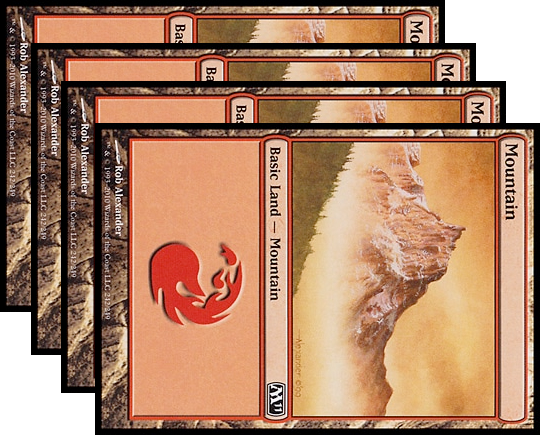
\includegraphics[width=0.33\textwidth]{picstcc/bf4.png}
    \vskip1ex
    $B_1$: ``Pensive Minotaur'' foi destruída, restam apenas as 3 Montanhas viradas usadas para jogá-la e a outra Montanha, virada, usada para jogar ``Flame Slash''.

    \vspace{.1cm}

    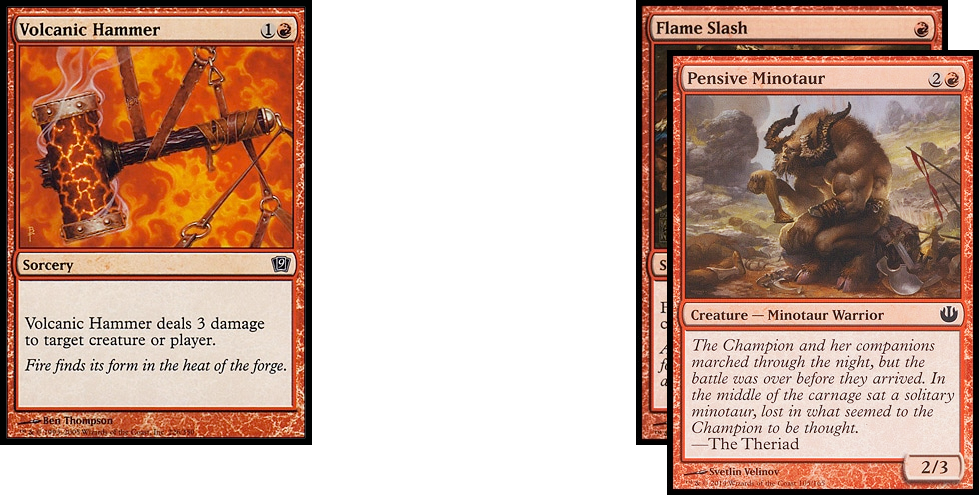
\includegraphics[width=0.6\textwidth]{picstcc/hand4.png}
    \vskip1ex
    $H$: A mão do agente consiste apenas em um feitiço ``Volcanic Hammer''. \\
    $G_1$: A pilha de descarte do agente, por sua vez, agora contém ambos o feitiço ``Flame Slash'' (quando um feitiço é usado, vai para a pilha de descarte) e a criatura ``Pensive Minotaur'' (destruída após o efeito de ``Flame Slash'' lhe causar dano maior ou igual à sua resistência).

    \vskip1ex
    A única ação legal em $s_4$ é passar para o final da fase:
    \begin{equation}
      A^P(s_4) := \begin{lrdcases}
                  Pass.
                  \end{lrdcases}
    \end{equation}
  \end{center}
\end{mdframed}

Apesar de ter um feitiço na mão, o agente não tem os recursos disponíveis para jogá-lo. Assim, a única ação legal é passar para a fase de combate, encerrando a primeira fase principal.
